% Workpiece frame to machine frame, including tool length
\documentclass[dvisvgm,tikz,border=4pt]{standalone}
% Shared preamble for the TikZ figures in images-1/src (compiled by build.sh)
\usepackage{helvet}
\renewcommand\familydefault{\sfdefault}
\usepackage{amsmath, amssymb}
\usetikzlibrary{arrows.meta, calc, decorations.pathreplacing, patterns, positioning, shapes.geometric, 3d, perspective, fit, backgrounds}
% palette shared with slides.scss and the Graphviz diagrams
\definecolor{dmred}{HTML}{880000}
\definecolor{dmblue}{HTML}{000088}
\definecolor{dmgreen}{HTML}{008800}
\definecolor{dmorange}{HTML}{E08A1E}
\definecolor{ink}{HTML}{333333}
\definecolor{fillblue}{HTML}{E8E8F8}
\definecolor{fillred}{HTML}{F3EAEA}
\definecolor{fillgreen}{HTML}{E8F4E8}
\definecolor{fillorange}{HTML}{FDF0DC}
\definecolor{steel}{HTML}{C9D3DC}
\definecolor{steeldk}{HTML}{8FA3B5}
\definecolor{metal}{HTML}{D9D9D9}
\definecolor{metaldk}{HTML}{A6A6A6}
\tikzset{
  >={Stealth[length=7pt]},
  every picture/.style={line cap=round, line join=round, font=\large},
  proj/.style={gray, dashed, thin},
  dim/.style={<->, >={Stealth[length=5pt]}, thin},
  ext/.style={very thin, gray},
  callout/.style={gray!70!black, thin},
  % datum (origin) symbol
  % pics use absolute sizes so they look the same in mm-scaled drawings
  datum/.pic={
    \fill[white] (0,0) circle (0.22cm);
    \fill[black] (0,0) -- ++(0.22cm,0) arc[start angle=0, end angle=-90, radius=0.22cm] -- cycle;
    \fill[black] (0,0) -- ++(-0.22cm,0) arc[start angle=180, end angle=90, radius=0.22cm] -- cycle;
    \draw[thick] (0,0) circle (0.22cm);
  },
  % reference symbols (absolute sizes): origins have a double circle with a filled quadrant
  wporigin/.pic={
    \draw[thick, fill=white] (0,0) circle (0.3cm);
    \fill[black] (0,0) -- (0.18cm,0) arc[start angle=0, end angle=-90, radius=0.18cm] -- cycle;
    \draw[thick] (0,0) circle (0.18cm);
    \draw (-0.3cm,0) -- (0.3cm,0) (0,-0.3cm) -- (0,0.3cm);
  },
  machorigin/.pic={
    \draw[thick, fill=white] (0,0) circle (0.3cm);
    \fill[black] (0,0) -- (-0.18cm,0) arc[start angle=180, end angle=90, radius=0.18cm] -- cycle;
    \draw[thick] (0,0) circle (0.18cm);
    \draw (-0.3cm,0) -- (0.3cm,0) (0,-0.3cm) -- (0,0.3cm);
  },
  supportpt/.pic={
    \draw[thick, fill=white] (0,0) circle (0.15cm);
    \draw (-0.15cm,0) -- (0.15cm,0) (0,-0.15cm) -- (0,0.15cm);
  },
  regpt/.pic={
    \draw[thick, fill=white] (0,0) circle (0.24cm);
    \draw[thick] (0,0) circle (0.15cm);
    \draw (-0.15cm,0) -- (0.15cm,0) (0,-0.15cm) -- (0,0.15cm);
  },
  % support / registration point (generic)
  target/.pic={
    \draw[thick, fill=white] (0,0) circle (0.12cm);
    \draw (-0.2cm,0) -- (0.2cm,0) (0,-0.2cm) -- (0,0.2cm);
  },
}

\begin{document}
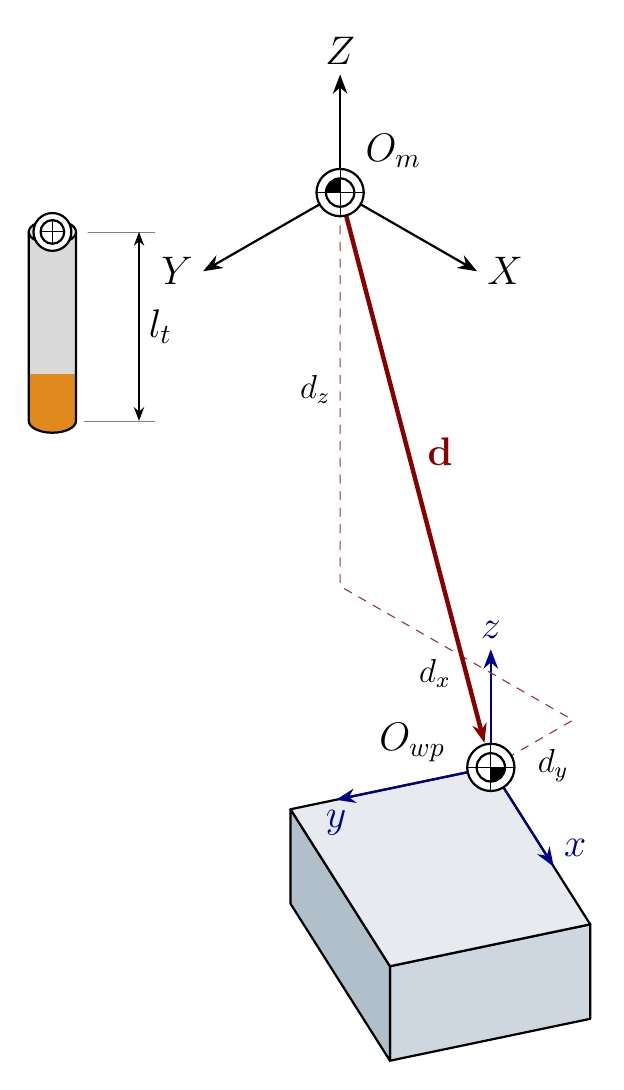
\begin{tikzpicture}[x={(0.87cm,-0.5cm)}, y={(-0.87cm,-0.5cm)}, z={(0cm,1cm)}, font=\Large]
  \coordinate (Om) at (0,0,5);       % machine origin
  \coordinate (Ow) at (3.4,1.2,0);   % workpiece origin
  \def\th{25}                        % workpiece rotation about z
  % workpiece block: top face at z=0, visible faces at x=3 and y=2.2 (local)
  \begin{scope}[shift={(Ow)}, rotate around z=\th]
    \filldraw[thick, fill=steel!90] (3,0,0) -- (3,2.2,0) -- (3,2.2,-1.2) -- (3,0,-1.2) -- cycle;
    \filldraw[thick, fill=steeldk!70] (0,2.2,0) -- (3,2.2,0) -- (3,2.2,-1.2) -- (0,2.2,-1.2) -- cycle;
    \filldraw[thick, fill=steel!45] (0,0,0) -- (3,0,0) -- (3,2.2,0) -- (0,2.2,0) -- cycle;
    \draw[->, thick, dmblue] (0,0,0) -- (1.9,0,0) node[above right] {$x$};
    \draw[->, thick, dmblue] (0,0,0) -- (0,1.7,0) node[below] {$y$};
    \draw[->, thick, dmblue] (0,0,0) -- (0,0,1.5) node[above] {$z$};
  \end{scope}
  \node[left=13pt, yshift=9pt] at (Ow) {$O_{wp}$};
  % machine frame
  \draw[->, thick] (Om) -- ++(2.0,0,0) node[right] {$X$};
  \draw[->, thick] (Om) -- ++(0,2.0,0) node[left] {$Y$};
  \draw[->, thick] (Om) -- ++(0,0,1.5) node[above] {$Z$};
  \node[above right=8pt] at (Om) {$O_m$};
  % components of d
  \draw[proj, dmred!80] (Om) -- node[left, black, font=\large] {$d_z$} (0,0,0)
     -- node[below left=-2pt, black, font=\large] {$d_x$} (3.4,0,0)
     -- node[below right=-2pt, black, font=\large] {$d_y$} (Ow);
  \draw[->, line width=1.6pt, dmred, shorten <=0.32cm, shorten >=0.32cm] (Om) -- node[pos=0.45, right=3pt] {$\mathbf{d}$} (Ow);
  % tool hanging from the spindle nose: registration point and length
  \begin{scope}[shift={(-1.6,2.6,5)}, x={(1cm,0cm)}, y={(0cm,1cm)}]
    \fill[metal] (-0.3,0) rectangle (0.3,-2.4);
    \fill[dmorange] (-0.3,-1.8) rectangle (0.3,-2.4);
    \fill[dmorange] (0,-2.4) ellipse [x radius=0.3, y radius=0.15];
    \draw[thick] (-0.3,0) -- (-0.3,-2.4) arc[start angle=180, end angle=360, x radius=0.3, y radius=0.15] -- (0.3,0);
    \filldraw[thick, fill=metal!60] (0,0) ellipse [x radius=0.3, y radius=0.15];
    \pic at (0,0) {regpt};
    \draw[ext] (0.45,0) -- (1.3,0) (0.4,-2.4) -- (1.3,-2.4);
    \draw[dim] (1.1,0) -- node[right] {$l_t$} (1.1,-2.4);
  \end{scope}
  % reference symbols on top of everything
  \pic at (Ow) {wporigin};
  \pic at (Om) {machorigin};
\end{tikzpicture}
\end{document}
